%%%%%%%%%%%%%%%%%%%%%%%%%%%%%%%%%%%%%%%%%%%%%%%%%%%%%%%%%%%%%%%%%%%%%%%%%%%%%%%%%%%%%%%%%%%%%%%%%
%
% Document:     Data Management  product tree
%
%%%%%%%%%%%%%%%%%%%%%%%%%%%%%%%%%%%%%%%%%%%%%%%%%%%%%%%%%%%%%%%%%%%%%%%%%%%%%%
\documentclass{article}
\usepackage{times,layouts}
\usepackage{tikz,hyperref,amsmath}
\usetikzlibrary{positioning,arrows,shapes,decorations.shapes,shapes.arrows}
\usetikzlibrary{backgrounds,calc}
\usepackage[paperwidth=52.0cm,paperheight=20.78cm,
left=-2mm,top=3mm,bottom=0mm,right=0mm,
noheadfoot,marginparwidth=0pt,includemp=false,
textwidth=30cm,textheight=50mm]{geometry}
\newcommand\showpage{%
\setlayoutscale{0.5}\setlabelfont{\tiny}\printheadingsfalse\printparametersfalse
\currentpage\pagedesign}
\hypersetup{pdftitle={DM products }, pdfsubject={Diagram illustrating the
                products in LSST DM }, pdfauthor={Autogenerated from MD}}
\tikzstyle{tbox}=[rectangle,text centered, text width=30mm]
\tikzstyle{wbbox}=[rectangle, rounded corners=3pt, draw=black, top color=blue!50!white,
                    bottom color=white, very thick, minimum height=12mm, inner sep=2pt,
                    text centered, text width=30mm]
\tikzstyle{pbox}=[rectangle, rounded corners=3pt, draw=black, top
 color=yellow!50!white, bottom color=white, very thick,
 minimum height=35pt, inner sep=2pt, text centered, text width=35mm]
\tikzstyle{pline}=[-, thick]
\begin{document}
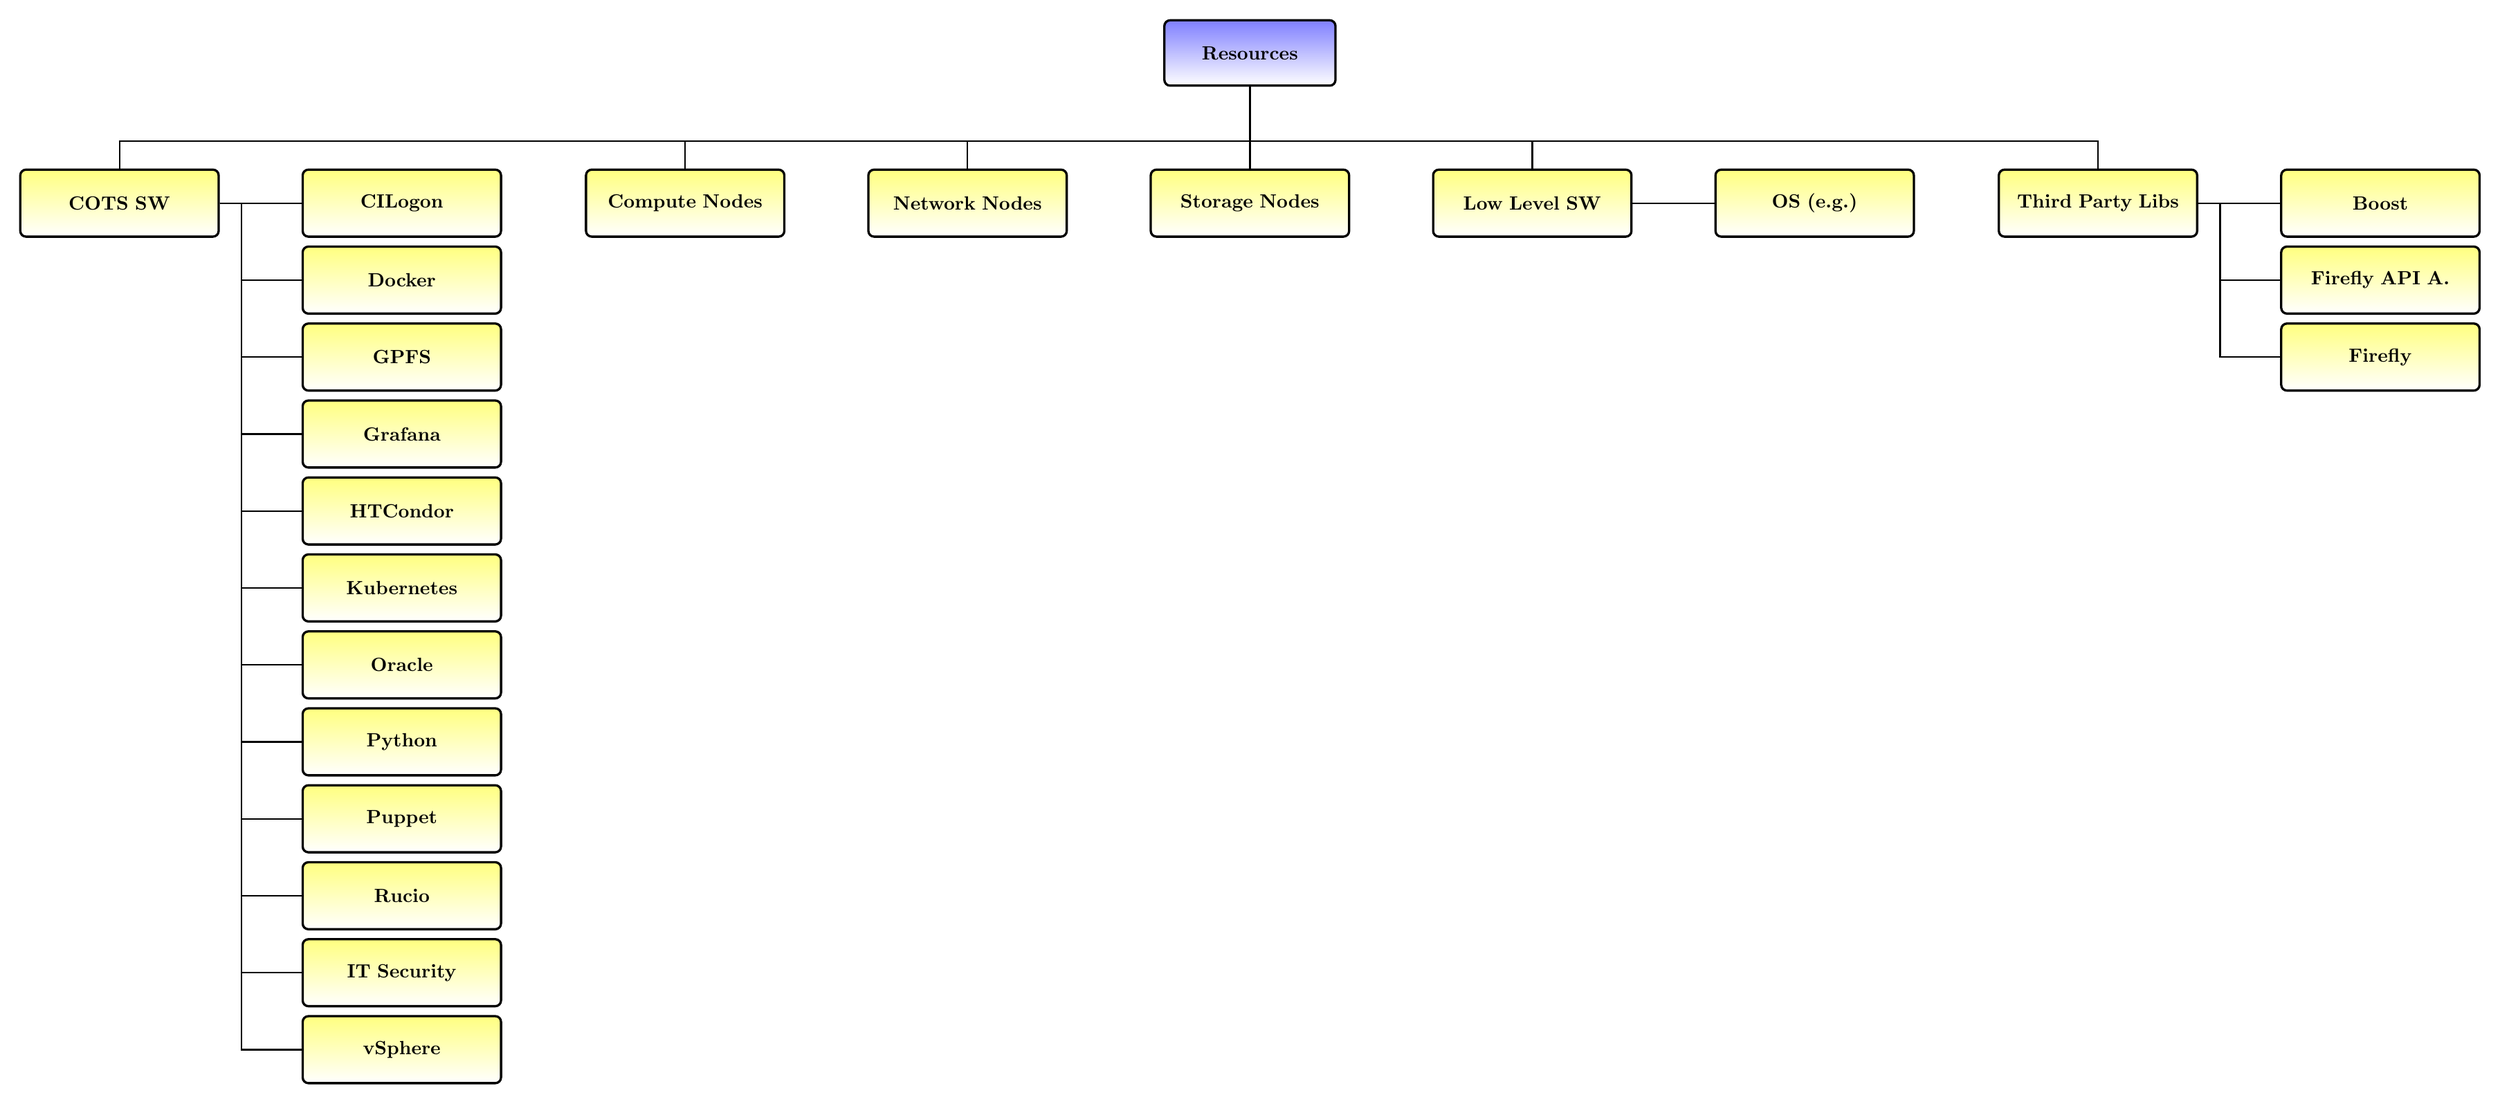
\begin{tikzpicture}[node distance=0mm]


\node (COTS) [pbox, 
] {\textbf{COTS SW
} };
\node (CILOGON) [pbox,right=15mm of COTS] {\textbf{CILogon
} };
 \draw[pline] (COTS.east) -| ++(0.4,0) |- (CILOGON.west); 
\node (DOCKER) [pbox,below=4pt of CILOGON] {\textbf{Docker
} };
 \draw[pline] (COTS.east) -| ++(0.4,0) |- (DOCKER.west); 
\node (GPFS) [pbox,below=4pt of DOCKER] {\textbf{GPFS
} };
 \draw[pline] (COTS.east) -| ++(0.4,0) |- (GPFS.west); 
\node (GRAFANA) [pbox,below=4pt of GPFS] {\textbf{Grafana
} };
 \draw[pline] (COTS.east) -| ++(0.4,0) |- (GRAFANA.west); 
\node (HTCONDOR) [pbox,below=4pt of GRAFANA] {\textbf{HTCondor
} };
 \draw[pline] (COTS.east) -| ++(0.4,0) |- (HTCONDOR.west); 
\node (K8S) [pbox,below=4pt of HTCONDOR] {\textbf{Kubernetes
} };
 \draw[pline] (COTS.east) -| ++(0.4,0) |- (K8S.west); 
\node (ORACLE) [pbox,below=4pt of K8S] {\textbf{Oracle
} };
 \draw[pline] (COTS.east) -| ++(0.4,0) |- (ORACLE.west); 
\node (PTH) [pbox,below=4pt of ORACLE] {\textbf{Python
} };
 \draw[pline] (COTS.east) -| ++(0.4,0) |- (PTH.west); 
\node (PUPPET) [pbox,below=4pt of PTH] {\textbf{Puppet
} };
 \draw[pline] (COTS.east) -| ++(0.4,0) |- (PUPPET.west); 
\node (RUCIO) [pbox,below=4pt of PUPPET] {\textbf{Rucio
} };
 \draw[pline] (COTS.east) -| ++(0.4,0) |- (RUCIO.west); 
\node (SECURITY) [pbox,below=4pt of RUCIO] {\textbf{IT Security
} };
 \draw[pline] (COTS.east) -| ++(0.4,0) |- (SECURITY.west); 
\node (VSPHERE) [pbox,below=4pt of SECURITY] {\textbf{vSphere
} };
 \draw[pline] (COTS.east) -| ++(0.4,0) |- (VSPHERE.west); 
\node (HWCOMP) [pbox, 
right=6.7cm of COTS] {\textbf{Compute Nodes
} };
\node (HWNET) [pbox, 
right=1.5cm of HWCOMP] {\textbf{Network Nodes
} };
\node (HWSTOR) [pbox, 
right=1.5cm of HWNET] {\textbf{Storage Nodes
} };
\node (LLSW) [pbox, 
right=1.5cm of HWSTOR] {\textbf{Low Level SW
} };
\node (CENTOS) [pbox,right=15mm of LLSW] {\textbf{OS (e.g.)
} };
 \draw[pline] (LLSW.east) -| ++(0.4,0) |- (CENTOS.west); 
\node (THPL) [pbox, 
right=6.7cm of LLSW] {\textbf{Third Party Libs
} };
\node (BOOST) [pbox,right=15mm of THPL] {\textbf{Boost
} };
 \draw[pline] (THPL.east) -| ++(0.4,0) |- (BOOST.west); 
\node (FFAA) [pbox,below=4pt of BOOST] {\textbf{Firefly API A.
} };
 \draw[pline] (THPL.east) -| ++(0.4,0) |- (FFAA.west); 
\node (FIREFLY) [pbox,below=4pt of FFAA] {\textbf{Firefly
} };
 \draw[pline] (THPL.east) -| ++(0.4,0) |- (FIREFLY.west); 
\node (HWCOTS) [wbbox, above=15mm of HWSTOR]{\textbf{Resources
}};
 \draw[pline]   (COTS.north) -- ++(0.0,0.5) -| (HWCOTS.south) ; 
 \draw[pline]   (HWCOMP.north) -- ++(0.0,0.5) -| (HWCOTS.south) ; 
 \draw[pline]   (HWNET.north) -- ++(0.0,0.5) -| (HWCOTS.south) ; 
 \draw[pline]   (HWSTOR.north) -- ++(0.0,0.5) -| (HWCOTS.south) ; 
 \draw[pline]   (LLSW.north) -- ++(0.0,0.5) -| (HWCOTS.south) ; 
 \draw[pline]   (THPL.north) -- ++(0.0,0.5) -| (HWCOTS.south) ; 

\end{tikzpicture}
\end{document}
